\section{Repr�sentations informatiques}

	\frame
	{
		\frametitle{Jeu de mains\ldots}
		
		\begin{block}{Exercice}
			Jusqu'\`a combien pouvez-vous compter avec vos $10$ doigts ?
		\end{block}
		
			\begin{block}{R\'eponse}
				1023 !
			\end{block}
		
	\begin{center}
		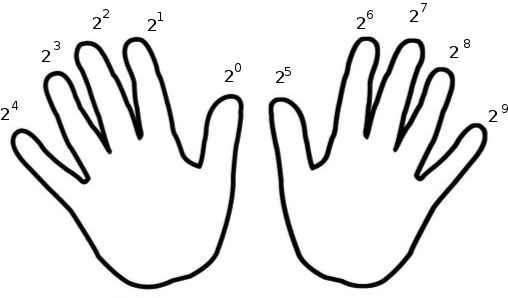
\includegraphics[width=.5\linewidth]{./figures/digits.png}
	\end{center}

	}
	
	\frame
	{
		\frametitle{Repr\'esentations num\'eriques}
		\begin{itemize}
			\item Repr\'esentation num\'erique : \emph{syst\`eme de num\'eration}.
			\item Syst\`eme de num\'eration connu, le \emph{d\'ecimal}, avec $10$ symboles :
			
			$0$ $1$ $2$ $3$ $4$ $5$ $6$ $7$ $8$ $9$
			\item Soit le nombre $199$ :
			
			$9\neq9$
			$\Rightarrow$ valeur d\'epend de la position : \emph{syst\`eme de num\'eration positionnel}.
			\item $0 \rightarrow 1\rightarrow  2 \rightarrow 3 \rightarrow 4 \rightarrow 5 \rightarrow 6 \rightarrow 7 \rightarrow 8 \rightarrow 9\rightarrow ?$ : on \emph{incr\'emente la position suivante} $\rightarrow 10$
			
			$10$ symboles $\Rightarrow$ \emph{base 10} : \emph{syst\`eme de num\'eration positionnel en base 10}.
		\end{itemize}
	}
	
	\frame
	{
		\frametitle{Notion de \emph{base}}
		
		Une repr\'esentation num\'erique doit \^etre adapt\'ee \`a ce qu'elle compte.
		\begin{itemize}
			\item Base $10$ : $10$ doigts.
			\item Autre base connue, $60$\ldots
			\item Informatique :
			\begin{itemize}
				\item base $2$,
				\item ou \emph{binaire},
				\item $0/1$, soit pas de courant/courant.
			\end{itemize}
		\end{itemize}
	}
	
	\frame
	{
		\frametitle{G\'en\'eralisation}
		\begin{block}{D\'efinition}
			Soit $x$ un nombre \`a $n$ chiffres dans le syst\`eme de num\'eration positionnel en base $b$.
			
			Alors $x$ s'\'ecrit
			
			$x_{n-1}x_{n-2}\ldots x_1x_0$
			
			et $x=\sum\limits_{i = 0}^{n-1}x_i\cdot b^i$.
		\end{block}
		
		Exemples :
		\begin{description}
			\item $2013_{10} = 2\cdot10^3 + 0\cdot10^2 + 1\cdot10^1+3\cdot10^0$
			\item $199_{10} = 1\cdot2^7 + 1\cdot2^6 + 0\cdot2^5+0\cdot2^4 + 0\cdot2^3 + 1\cdot2^2 + 1\cdot2^1+1\cdot2^0 = 11000111_2$
		\end{description}
	}

\frame
{
	\frametitle{Little ou Big Endian}
	\begin{itemize}
		\item Origines chaotiques de l�informatique.
		\item Diff�rents ordres de stockage pour les valeurs encod�es sur plusieurs octets (1 octet = 8 bits = $2^8$ possibilit�s = 256 valeurs).
		\begin{itemize}
			\item Little Endian : moins importants en dernier.
			\item Big Endian : plus importants en dernier.
		\end{itemize}
		\item Exemple avec l�entier 2012 :
		\begin{itemize}
			\item Sur 2 octets
			\begin{itemize}
				\item Little Endian : 0x07DC
				\item Big Endian : 0xDC07
			\end{itemize}
			\item Sur 4 octets
			\begin{itemize}
				\item Little Endian : 0x000007DC
				\item Big Endian : 0xDC070000
			\end{itemize}
		\end{itemize}
	\end{itemize}
}
